\documentclass{beamer}
\usepackage{listings}
\lstset{
%language=C,
frame=single, 
breaklines=true,
columns=fullflexible
}
\usepackage{subcaption}
\usepackage{url}
\usepackage{amsmath}

\usepackage{amsthm}

\usepackage{tikz}
\usepackage{graphicx}
\usepackage{tkz-euclide} % loads  TikZ and tkz-base
%\usetkzobj{all}
\usetikzlibrary{calc,math}
\usepackage{float}

\newcommand\norm[1]{\left\lVert#1\right\rVert}
\renewcommand{\vec}[1]{\mathbf{#1}}
\newcommand{\R}{\mathbb{R}}
\newcommand{\C}{\mathbb{C}}
\providecommand{\brak}[1]{\ensuremath{\left(#1\right)}}
\providecommand{\abs}[1]{\vert#1\vert}
\providecommand{\fourier}{\overset{\mathcal{F}}{ \rightleftharpoons}}
\newcommand{\myvec}[1]{\ensuremath{\begin{pmatrix}#1\end{pmatrix}}}
\providecommand{\mean}[1]{E[ #1 ]}
\providecommand{\sbrak}[1]{\ensuremath{{}\left[#1\right]}}
\providecommand{\cbrak}[1]{\ensuremath{\left\{#1\right\}}}
\usepackage[export]{adjustbox}
\usepackage[utf8]{inputenc}
\usepackage{amsmath}
\usetheme{Boadilla}
\title{Determine Earthquake Probability Based on Linear Regression Algorithm}
\author{Savarana Datta }
\institute{AI20BTECH11008}
\date{\today}

\begin{document}
\begin{frame}{}
 \titlepage 
\end{frame}
\begin{frame}{Introduction}
Natural Disaster (such as Earthquake) is an appearance that occurs when compatibility of nature is broken and that causes destruction of lives and properties; in this regard earthquake probability is a big deal for our life.
\end{frame}

\begin{frame}{Key words}
$\bullet$Earthquake (EQ)\\
$\bullet$Earthquake probability (EQP)\\
$\bullet$Earthquake probability using linear regression (LR-EQP)\\
$\bullet$combustible elements (CE)\\
$\bullet$Latitude and Longitude (Lat-Long)\\
$\bullet$Tectonic plate (TP)\\
$\bullet$Soil type (ST)\\
$\bullet$Density of population (DP).
\end{frame}

\begin{frame}{}
Our main motive for this work is:\\
$\bullet$To manage data mining for geological issues.\\
$\bullet$To create strong connection between geological data and data mining.\\
$\bullet$To reduce the disastrous effect by getting information about disaster before.
\end{frame}
\begin{frame}{Data Mining}
The earthquake prediction using data mining use 3 factors these are:
$\bullet$Ground water levels.\\
$\bullet$Chemical changes in ground water. \\
$\bullet$Radon gas in ground water wells.
\end{frame}

\begin{frame}{Earthquake probability using linear regression (LR-EQP)}
LR-EQP uses five the attributes which are related geologically: \\
$\bullet$Latitude and Longitude of location.\\
$\bullet$Combustible Elements.\\
$\bullet$Density of Population.\\
$\bullet$Distance from nearest TP.\\
$\bullet$Soil type.
\end{frame}
\begin{frame}{Flow Chart of LR-EQP}
    \begin{figure}[h]
    \centering
    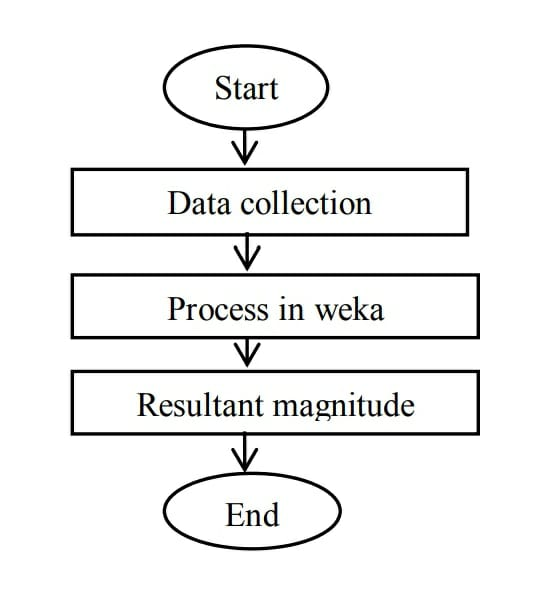
\includegraphics[width=0.5\textwidth]{P1.jpeg}
\end{figure} 

\end{frame}
 \begin{frame}{}
 Step-1:Data Collection:\\
 $\bullet$Latitude-Longitude\\
 $\bullet$CE is also responsible as the TPs can rubbing with each other and create a huge temperature.\\
 $\bullet$DP measure the pressure on the surface.\\
 $\bullet$Soil Type.\\
\end{frame}
\begin{frame}{}
Step-2:Process in weka:\\
$\bullet$All the data of the attributes are collected in a excel file.\\
$\bullet$The excel file is converted into CSV file.\\
$\bullet$Weka use this CSV file for preprocessing data, select attribute, choose coherent attribute and remove incoherent attribute(classification and assessment).\\
$\bullet$After preprocessing data file LR-EQP is implemented through linear regression.\\
$\bullet$The training data set which is get from weka is used for further measurement of magnitude for EQ.\\
 \end{frame}
 \begin{frame}
   \begin{figure}[h]
    \centering
    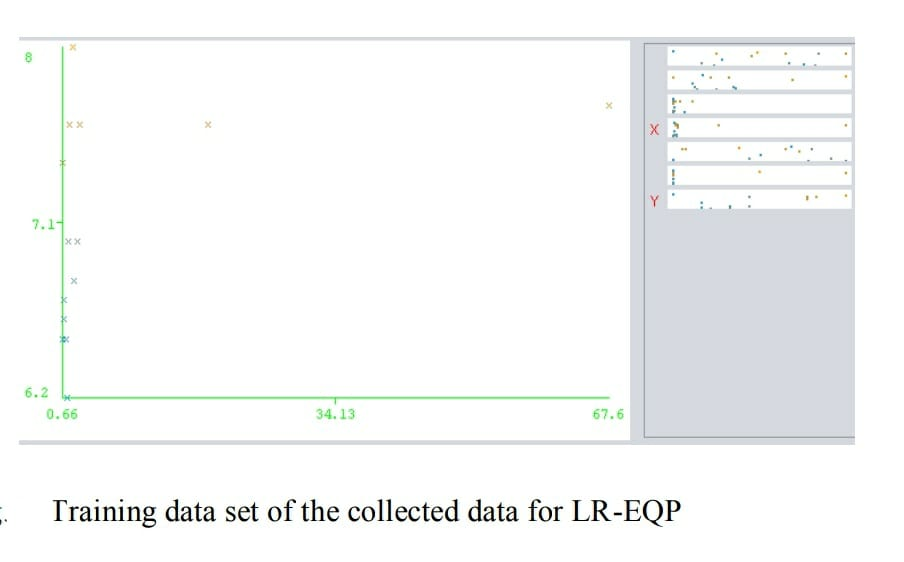
\includegraphics[width=0.8\textwidth]{P3.jpeg}
\end{figure}   
 \end{frame}
 \begin{frame}{}
 Step-3:Resultant magnitude:\\
 $\bullet$After getting the training data set from weka, it is used as a model for getting the magnitude for EQ.\\
 $\bullet$Before getting the magnitude of an area LR-EQP needed to be given another agnitude of the relevant area which is the magnitude of previous EQ.\\
 $\bullet$Without this manually given magnitude the resultant magnitude cannot be acquired.\\
 
\end{frame}
\begin{frame}{}
   \begin{figure}[h]
    \centering
    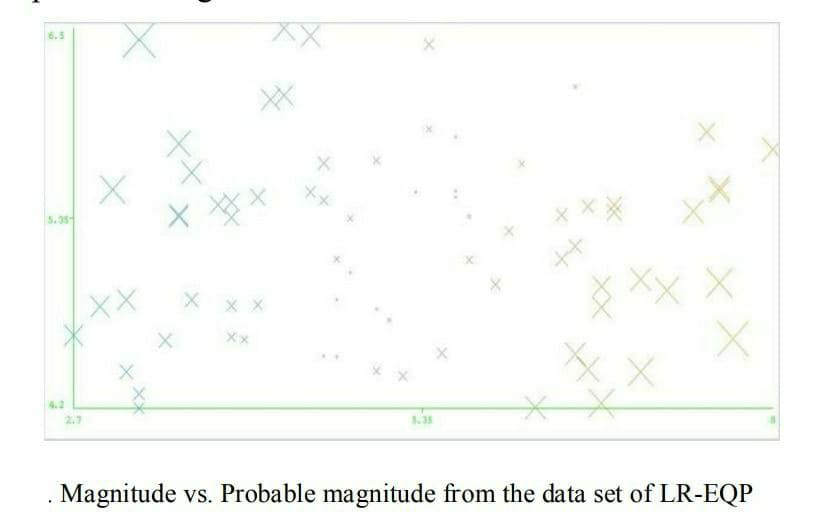
\includegraphics[width=0.8\textwidth]{P2.jpeg}
\end{figure}  
\end{frame}
\begin{frame}{Experimental Analysis}
\textbf{A.Experimental Setup}:\\
LR-EQP has been developed in Weka for preparing a model which is further implemented in Android studio.We get an APK file from android studio.The APK file gives the probable magnitude for that relevant area.\\
\end{frame}
\begin{frame}{}
  \textbf{B.Experimental Result and Comparisons:}\\
  \begin{figure}[h]
    \centering
    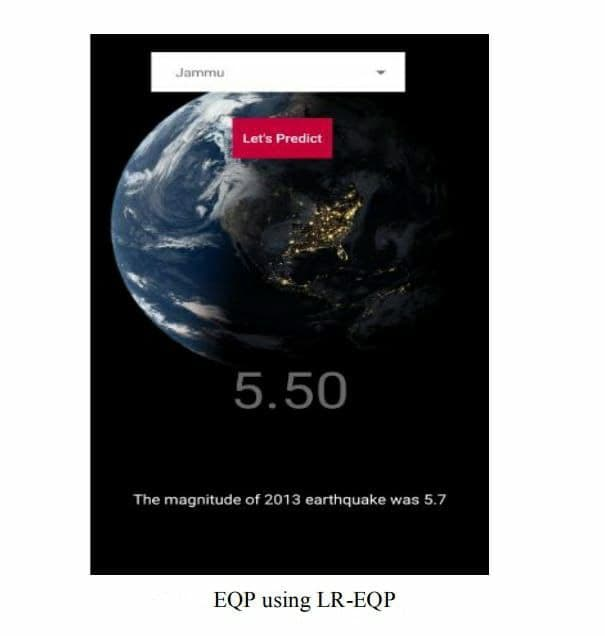
\includegraphics[width=0.6\textwidth]{P5.jpg}
\end{figure}  
\end{frame}
\begin{frame}{}
LR-EQP uses data of Jammu region earlier 5 years of 2013 and give the result of magnitude 5.5. There was an EQ in Jammu in 2013 and the magnitude of that EQ was 5.7.\\
The experimental results presented in the above section can measure the magnitude and gives output near about original magnitude.\\
 \begin{figure}[h]
    \centering
    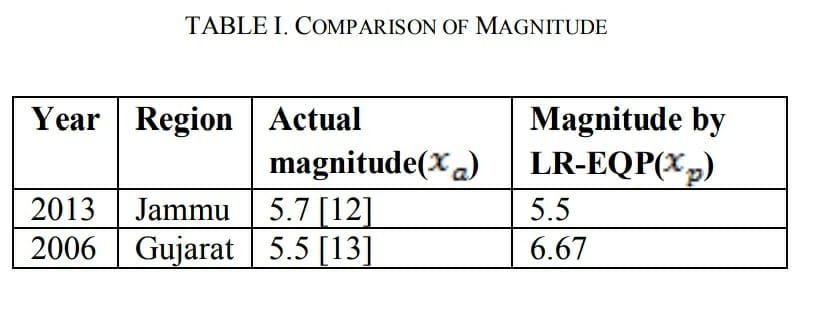
\includegraphics[width=0.8\textwidth]{P4.jpeg}
\end{figure}

\end{frame}
\begin{frame}{}
  The fluctuation of magnitude from the original magnitude can be calculated with standard deviation.\\
\begin{align}
sd &=\sqrt{\frac{\sum(x_{\alpha}-x_{p})^{2}}{n-1}}\\
   &=\sqrt{\frac{(5.7-5.5)^{2}+(5.5-6.67)^{2}}{2-1}}\\
   &=1.4089
\end{align}
Here in LR-EQP the standard deviation is 1.4089 which indicates that the data set for LR-EQP is close to the expected value. 
\end{frame}
\end{document}
